% Anhui 2011 solid schematic: A-O-D dashed, C-O-E dashed, spokes dashed, outer solid.
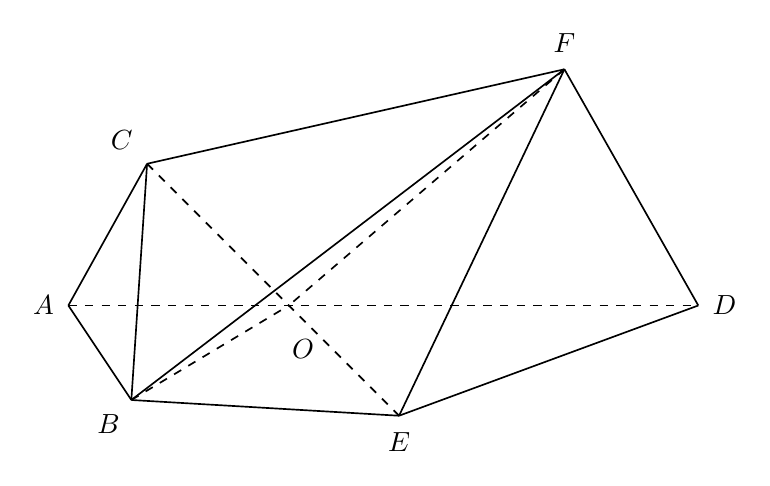
\begin{tikzpicture}[x=1cm,y=1cm,font=\normalsize,
  geometry edge/.style={draw=black,solid,line width=.6pt},
  geometry hidden/.style={draw=black,dashed,line width=.6pt},
  geometry label/.style={font=\normalsize,inner sep=2pt,fill=white}]
\coordinate (A) at (0.0,1.6);
\coordinate (O) at (2.8,1.6);
\coordinate (D) at (8.0,1.6);
\coordinate (C) at (1.0,3.4);
\coordinate (E) at (4.2,0.2);
\coordinate (B) at (0.8,0.4);
\coordinate (F) at (6.3,4.6);
% hidden: AD and CE and spokes
\draw[geometry hidden] (A)--(O)--(D);
\draw[geometry hidden] (C)--(O)--(E);
\draw[geometry hidden] (B)--(O);
\draw[geometry hidden] (F)--(O);
% solid outer and faces
\draw[geometry edge] (A)--(B);
\draw[geometry edge] (A)--(C);
\draw[geometry edge] (B)--(C);
\draw[geometry edge] (B)--(E);
\draw[geometry edge] (E)--(D);
\draw[geometry edge] (D)--(F);
\draw[geometry edge] (C)--(F);
\draw[geometry edge] (E)--(F);
\draw[geometry edge] (B)--(F);
\node[geometry label,left,xshift=-3pt] at (A) {$A$};
\node[geometry label,below left,xshift=-2pt,yshift=-3pt] at (B) {$B$};
\node[geometry label,above left,xshift=-3pt,yshift=3pt] at (C) {$C$};
\node[geometry label,below right,xshift=5pt,yshift=-6pt,fill=none,xshift=-6.00bp,yshift=-4.00bp] at (O) {$O$};
\node[geometry label,right,xshift=3pt] at (D) {$D$};
\node[geometry label,below,yshift=-4pt] at (E) {$E$};
\node[geometry label,above,yshift=4pt] at (F) {$F$};
\end{tikzpicture}